% this file is called up by thesis.tex
% content in this file will be fed into the main document

%: ----------------------- name of chapter  -------------------------
\chapter{Conclusion} % top level followed by section, subsection


%: ----------------------- paths to graphics ------------------------

% change according to folder and file names
\ifpdf
    \graphicspath{{X/figures/PNG/}{X/figures/PDF/}{X/figures/}}
\else
    \graphicspath{{X/figures/EPS/}{X/figures/}}
\fi

%: ----------------------- contents from here ------------------------

\section{Future Work}

This paper discusses various kinds of issue regarding to the development of 
HCMP Player, the HCMP Player itself is part of a larger HCMP project 
that facilitates music representation, preparation, and performance,
and there are some components can be built upon HCMP Player and some 
can be directly intergrate with HCMP Player. Two
features can be added to further extend the HCMP Player's function. 

\subsection{Integrate with Score Following}
HCMP has a score following component which is also developed with serpent.
Figure 7.1 is a screenshot of score following component. The score following component 
can be used to notate music score, turning 
``pages''. The original score following component has a builtin player function,
and it can easily replaced by HCMP Player. With predefined API of HCMP Player,  
score following component can be easily extended to cooperate with HCMP Plyaer.
The HCMP Player will synchronize with score following componet by constantly 
receiving command through network. 

\begin{figure}[H]
\center{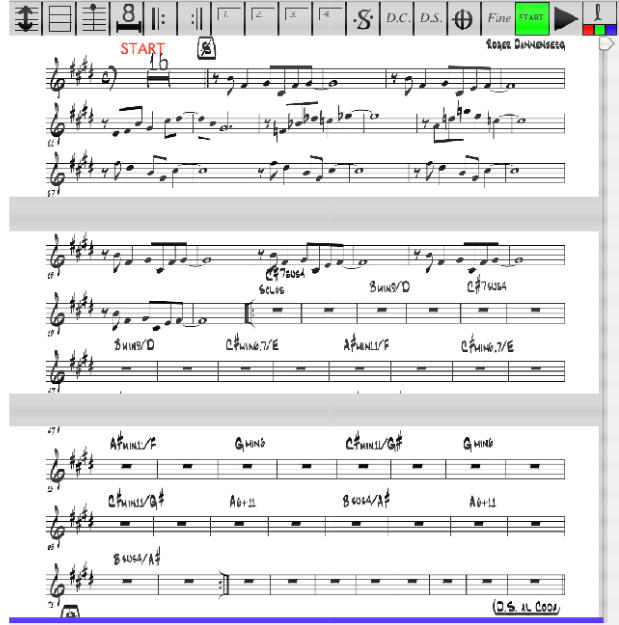
\includegraphics[width=0.5\linewidth]{8/1.png}}
\caption{HCMP Score Display Component}
\label{fig:speciation}
\end{figure}

\subsection{Integraet with Midi Database}
Another interesting work is about midi database\cite{Dawen:ISMIR2011} which 
is based on Dawen Liang's previous work. The basic idea of midi database 
is to create a tool by which user is able to quickly record, organize
and retrieve audio information from various sources. The midi database 
define a full set of API for its clients. One possible extention of HCMP 
Player is to integrate midi database into HMCP Player library function, 
so that user can easily use HCMP Player to search and play midi 
segement from previous history database.

\section{Conclusion}
From HCMP project's perspective, HCMP Player is a building block of a larger
project, upon which more powerful component can be built, it can also 
cooperate with other components to complete complex job, or be used by other
components. From developer's 
perspective, HCMP Player provides a complete set of API which can be extended 
and tailored to fit into more sophiscated project.
The HCMP Player can be split into 3 parts,  
GUI, player engine and network. The design and usage of each part 
is explained in detail in previous chapters. I also briefly decribe 
implementation of each part, as supplementary,
some pseucode segment is provide to illustrate logic. At the end, complete 
HCMP Player features is listed and a successful criteria is defined to
help evaluate the project.
